\documentclass[journal,12pt,twocolumn]{IEEEtran}
%
\usepackage{setspace}
\usepackage{gensymb}
\usepackage{siunitx}
\usepackage{tkz-euclide} 
\usepackage{textcomp}
\usepackage{standalone}
\usetikzlibrary{calc}
\newcommand\hmmax{0}
\newcommand\bmmax{0}

%\doublespacing
\singlespacing

%\usepackage{graphicx}
%\usepackage{amssymb}
%\usepackage{relsize}
\usepackage[cmex10]{amsmath}
%\usepackage{amsthm}
%\interdisplaylinepenalty=2500
%\savesymbol{iint}
%\usepackage{txfonts}
%\restoresymbol{TXF}{iint}
%\usepackage{wasysym}
\usepackage{amsthm}
%\usepackage{iithtlc}
\usepackage{mathrsfs}
\usepackage{txfonts}
\usepackage{stfloats}
\usepackage{bm}
\usepackage{cite}
\usepackage{cases}
\usepackage{subfig}
%\usepackage{xtab}
\usepackage{longtable}
\usepackage{multirow}
%\usepackage{algorithm}
%\usepackage{algpseudocode}
\usepackage{enumitem}
\usepackage{mathtools}
\usepackage{steinmetz}
\usepackage{tikz}
\usepackage{circuitikz}
\usepackage{verbatim}
\usepackage{tfrupee}
\usepackage[breaklinks=true]{hyperref}
%\usepackage{stmaryrd}
\usepackage{tkz-euclide} % loads  TikZ and tkz-base
%\usetkzobj{all}
\usetikzlibrary{calc,math}
\usepackage{listings}
    \usepackage{color}                                            %%
    \usepackage{array}                                            %%
    \usepackage{longtable}                                        %%
    \usepackage{calc}                                             %%
    \usepackage{multirow}                                         %%
    \usepackage{hhline}                                           %%
    \usepackage{ifthen}                                           %%
  %optionally (for landscape tables embedded in another document): %%
    \usepackage{lscape}     
\usepackage{multicol}
\usepackage{chngcntr}
\usepackage{amsmath}
\usepackage{cleveref}
\usepackage{amsmath}
%\usepackage{enumerate}

%\usepackage{wasysym}
%\newcounter{MYtempeqncnt}
\DeclareMathOperator*{\Res}{Res}
%\renewcommand{\baselinestretch}{2}
\renewcommand\thesection{\arabic{section}}
\renewcommand\thesubsection{\thesection.\arabic{subsection}}
\renewcommand\thesubsubsection{\thesubsection.\arabic{subsubsection}}

\renewcommand\thesectiondis{\arabic{section}}
\renewcommand\thesubsectiondis{\thesectiondis.\arabic{subsection}}
\renewcommand\thesubsubsectiondis{\thesubsectiondis.\arabic{subsubsection}}

% correct bad hyphenation here
\hyphenation{op-tical net-works semi-conduc-tor}
\def\inputGnumericTable{}                                 %%

\lstset{
%language=C,
frame=single, 
breaklines=true,
columns=fullflexible
}
%\lstset{
%language=tex,
%frame=single, 
%breaklines=true
%}
\usepackage{graphicx}
\usepackage{pgfplots}

\begin{document}


\newtheorem{theorem}{Theorem}[section]
\newtheorem{problem}{Problem}
\newtheorem{proposition}{Proposition}[section]
\newtheorem{lemma}{Lemma}[section]
\newtheorem{corollary}[theorem]{Corollary}
\newtheorem{example}{Example}[section]
\newtheorem{definition}[problem]{Definition}
%\newtheorem{thm}{Theorem}[section] 
%\newtheorem{defn}[thm]{Definition}
%\newtheorem{algorithm}{Algorithm}[section]
%\newtheorem{cor}{Corollary}
\newcommand{\BEQA}{\begin{eqnarray}}
\newcommand{\EEQA}{\end{eqnarray}}
\newcommand{\define}{\stackrel{\triangle}{=}}
\bibliographystyle{IEEEtran}
%\bibliographystyle{ieeetr}
\providecommand{\mbf}{\mathbf}
\providecommand{\abs}[1]{\ensuremath{\left\vert#1\right\vert}}
\providecommand{\norm}[1]{\ensuremath{\left\lVert#1\right\rVert}}
\providecommand{\mean}[1]{\ensuremath{E\left[ #1 \right]}}
\providecommand{\pr}[1]{\ensuremath{\Pr\left(#1\right)}}
\providecommand{\qfunc}[1]{\ensuremath{Q\left(#1\right)}}
\providecommand{\sbrak}[1]{\ensuremath{{}\left[#1\right]}}
\providecommand{\lsbrak}[1]{\ensuremath{{}\left[#1\right.}}
\providecommand{\rsbrak}[1]{\ensuremath{{}\left.#1\right]}}
\providecommand{\brak}[1]{\ensuremath{\left(#1\right)}}
\providecommand{\lbrak}[1]{\ensuremath{\left(#1\right.}}
\providecommand{\rbrak}[1]{\ensuremath{\left.#1\right)}}
\providecommand{\cbrak}[1]{\ensuremath{\left\{#1\right\}}}
\providecommand{\lcbrak}[1]{\ensuremath{\left\{#1\right.}}
\providecommand{\rcbrak}[1]{\ensuremath{\left.#1\right\}}}
\theoremstyle{remark}
\newtheorem{rem}{Remark}
\newcommand{\sgn}{\mathop{\mathrm{sgn}}}
\providecommand{\res}[1]{\Res\displaylimits_{#1}} 
%\providecommand{\norm}[1]{\lVert#1\rVert}
\providecommand{\mtx}[1]{\mathbf{#1}}
\providecommand{\fourier}{\overset{\mathcal{F}}{ \rightleftharpoons}}
%\providecommand{\hilbert}{\overset{\mathcal{H}}{ \rightleftharpoons}}
\providecommand{\system}{\overset{\mathcal{H}}{ \longleftrightarrow}}
	%\newcommand{\solution}[2]{\textbf{Solution:}{#1}}
\newcommand{\solution}{\noindent \textbf{Solution: }}
\newcommand{\cosec}{\,\text{cosec}\,}
\providecommand{\dec}[2]{\ensuremath{\overset{#1}{\underset{#2}{\gtrless}}}}
\newcommand{\myvec}[1]{\ensuremath{\begin{pmatrix}#1\end{pmatrix}}}
\newcommand{\mydet}[1]{\ensuremath{\begin{vmatrix}#1\end{vmatrix}}}
%\numberwithin{equation}{section}
\numberwithin{equation}{subsection}
%\numberwithin{problem}{section}
%\numberwithin{definition}{section}
\makeatletter
\@addtoreset{figure}{problem}
\makeatother
\let\StandardTheFigure\thefigure
\let\vec\mathbf
%\renewcommand{\thefigure}{\theproblem.\arabic{figure}}
\renewcommand{\thefigure}{\theproblem}
%\setlist[enumerate,1]{before=\renewcommand\theequation{\theenumi.\arabic{equation}}
%\counterwithin{equation}{enumi}
%\renewcommand{\theequation}{\arabic{subsection}.\arabic{equation}}
\def\putbox#1#2#3{\makebox[0in][l]{\makebox[#1][l]{}\raisebox{\baselineskip}[0in][0in]{\raisebox{#2}[0in][0in]{#3}}}}
     \def\rightbox#1{\makebox[0in][r]{#1}}
     \def\centbox#1{\makebox[0in]{#1}}
     \def\topbox#1{\raisebox{-\baselineskip}[0in][0in]{#1}}
\vspace{3cm}
\title{Bayesian Linear Regression- (Parameter distribution)}
\maketitle
\newpage
%\tableofcontents
\bigskip
\renewcommand{\thefigure}{\theenumi}
\renewcommand{\thetable}{\theenumi}
\begin{abstract}
This document contains theory behind curve fitting model
\end{abstract}
\section{\textbf{Objective}}
Our objective is to implement the parameter distribution  implemention from scratch.
\section{Load Dataset}
Create a sinusoidal data function
\begin{align}
    y = A\sin{2\pi{ft}}+n\brak{t}
\end{align}
with random noise included in the target values training set comprising N observations of t,
written
\begin{align}
    t=\myvec{t_1 &,&.&.& t_N}^T 
\end{align}
together with corresponding observations of the values
of y, denoted 
\begin{align}
    y=\myvec{y_1 &,&.&.& y_N}^T
\end{align}
\begin{figure}[!h]
\begin{center}
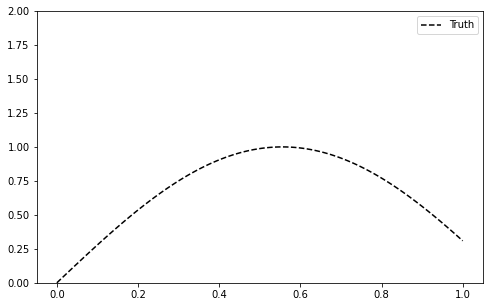
\includegraphics[width=3.4in]{a1.png}
\end{center}
\caption{Sinusoidal Dataset}
\label{fig:1}
\end{figure}
Fig \ref{fig:1} was generated by choosing
values of $t_n$, for n = 1, . . . , N, where N= 20 and spaced randomly. Data set y was obtained by first computing the corresponding values of the function $A\sin2\pi{ft}$ and then adding a small level of random noise having a random distribution to each such point in order to obtain the corresponding value.
\begin{lstlisting}
def create_data(t, noise_variance):
    return np.sin(0.9*np.pi*t) + noise(t.shape, noise_variance)

def noise(size, variance):
    return np.random.normal(scale=np.sqrt(variance), size=size)
\end{lstlisting}
From the above code we will get $\phi$ matrix of size (20,11) . Here column-1 will always be the value of coefficient, which will always be 1. But to create a matrix we need to consider it as a column.
\begin{align}
\phi= \myvec{ 1 & t_{0} & t_{0}^2 & \ldots & t_{0}^{N-1} \\
		1 & t_{1} & t_{1}^2 & \ldots & t_{1}^{N-1} \\
		1 & t_{2} & t_{2}^2 & \ldots & t_{2}^{N-1} \\
		\vdots & & \vdots &  & \vdots  \\
		    1 & \ldots & \ldots & \ldots & t_{N}^{N-1} }\label{eq:1}
\end{align}
\section{Parameter distribution}
For a Bayesian treatment of linear regression we need a prior probability distribution over model parameters $\vec{w}$. For reasons of simplicity, we will use an isotropic Gaussian distribution over parameters $\vec{w}$ with zero mean.
%
\begin{align}
p\brak{\vec{w}\lvert \alpha} = \mathcal{N}\brak{\mathbf{w} \lvert \mathbf{0}, \alpha^{-1}\mathbf{I}}
\end{align}
%
An isotropic Gaussian distribution has a diagonal covariance matrix where all diagonal elements have the same variance $\alpha^{-1}$ \brak{$\alpha$ is the precision of the prior}. A zero mean favors smaller values of parameters $\vec{w_j}$ a priori. The prior is conjugate to the likelihood $p(\vec{t} \lvert \vec{w}, \beta)$ meaning that the posterior distribution has the same functional form as the prior i.e. is also a Gaussian. In this special case, the posterior has an analytical solution with the following sufficient statistics.
\begin{align}
\vec{m}_N &= \beta \vec{S}_N \boldsymbol\Phi^T \vec{t} \label{eq:2}\\
\vec{S}_N^{-1} &= \alpha\vec{I} + \beta \boldsymbol\Phi^T \boldsymbol\Phi \label{eq:3}
\end{align}
\eqref{eq:2} is the mean vector of the posterior and \eqref{eq:3} the inverse covariance matrix. Hence, the posterior distribution can be written as
\begin{align}
    p(\mathbf{w} \lvert \mathbf{t}, \alpha, \beta) = \mathcal{N}(\mathbf{w} \lvert \mathbf{m}_N, \mathbf{S}_N) \label{eq:5}
\end{align}

For the moment, we assume that the values of $\alpha$ and $\beta$ are known. Since the posterior is proportional to the product of likelihood and prior, the log of the posterior distribution is proportional to the sum of the log likelihood and the log of the prior
\begin{align}
    \log p(\mathbf{w} \lvert \mathbf{t}, \alpha, \beta) = 
-\beta E_D(\mathbf{w}) - \alpha E_W(\mathbf{w}) + \mathrm{const.} \label{eq:6}
\end{align}
\begin{lstlisting}

def posterior(Phi, t, alpha, beta, return_inverse=False):
    S_N_inv = alpha * np.eye(Phi.shape[1]) + beta * Phi.T.dot(Phi)
    S_N = np.linalg.inv(S_N_inv)
    m_N = beta * S_N.dot(Phi.T).dot(t)
    if return_inverse:
        return m_N, S_N, S_N_inv
    else:
        return m_N, S_N
\end{lstlisting}
Plot the posterior and actual data.
\begin{lstlisting}
def plot_data(x, t):
    plt.scatter(x, t, marker='o', c="k", s=20)


def plot_truth(x, y, label='Truth'):
    plt.plot(x, y, 'k--', label=label)


def plot_posterior_samples(x, ys, plot_xy_labels=True):
    plt.plot(x, ys[:, 0], 'r-', alpha=0.5, label='Post. samples')
    for i in range(1, ys.shape[1]):
        plt.plot(x, ys[:, i], 'r-', alpha=0.5)

    if plot_xy_labels:
        plt.xlabel('x')
        plt.ylabel('y')

\end{lstlisting}
\begin{figure}[!h]
\begin{center}
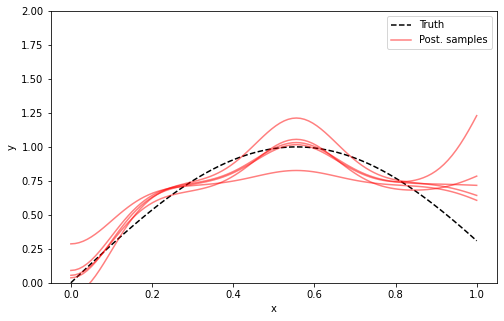
\includegraphics[width=3.4in]{a2.png}
\end{center}
\caption{Sinusoidal Dataset}
\label{fig:1}
\end{figure}
Download Python codes from 
%
\begin{lstlisting}
https://github.com/ayushkesh/EE4015/tree/master/A5
\end{lstlisting}
\end{document}